%==================================================%
% Basic setup starts here
%==================================================%
\documentclass[12pt, letterpaper]{amsart} % this will automatically load amsmath and amsthm packages
\usepackage{amsfonts}
\usepackage{amscd} % a CD environment for commutative rectangular diagram
\usepackage{mathtools} % for \shortintertext
\usepackage[utf8]{inputenc} % encoding method
\usepackage[mathscr]{eucal} % eucal calligraphy, mathsrc = use \mathcal
\usepackage{indentfirst} % indent first line of all sections
\usepackage{graphicx} % extension of graphics, options for \includegrahpicx
\usepackage{pict2e} % new implementation of the picture environment, which allows programming pictures directly LaTeX
\usepackage{epic} % add some command to the picture environment
\usepackage[margin=2.9cm]{geometry} % customize page layout
\usepackage{glossaries}

%==================================================%
% Additional setup ends here
%==================================================%
% Additional package used for relevant article
\usepackage{physics} % partial derivative \pdv
\usepackage{cleveref} % automatically add eq in referencing
\usepackage{cancel}
\usepackage{tikz}
\usepackage{graphicx}
\graphicspath{ {images/} }

% SELF-DEFINED THEOREM using amsthm package
\newtheorem{Th}{Theorem}[section]
\numberwithin{equation}{section}
\newtheorem{Def}[Th]{Definition}


%==================================================%
% Glossary
%==================================================%
%==================================================%
% Document starts here
% ==================================================%
\author{Kin Chang \\Co-Author: 
Amir Omidfar}
\title{2 wheel robot Derivation}
\begin{document}
\maketitle
\pagebreak
\tableofcontents
\pagebreak
\section*{Lab Overview:}
This lab derives a mathematical input-output model of the system dynamics based on a model of sensor and actuator responses for a two wheel car. Using this model in computational environment it would then create a state estimator for the location of the car in a 4 wall bounding open space. State estimator follows extended Kalman filter procedure to derive required results.



\begin{figure}[h!]
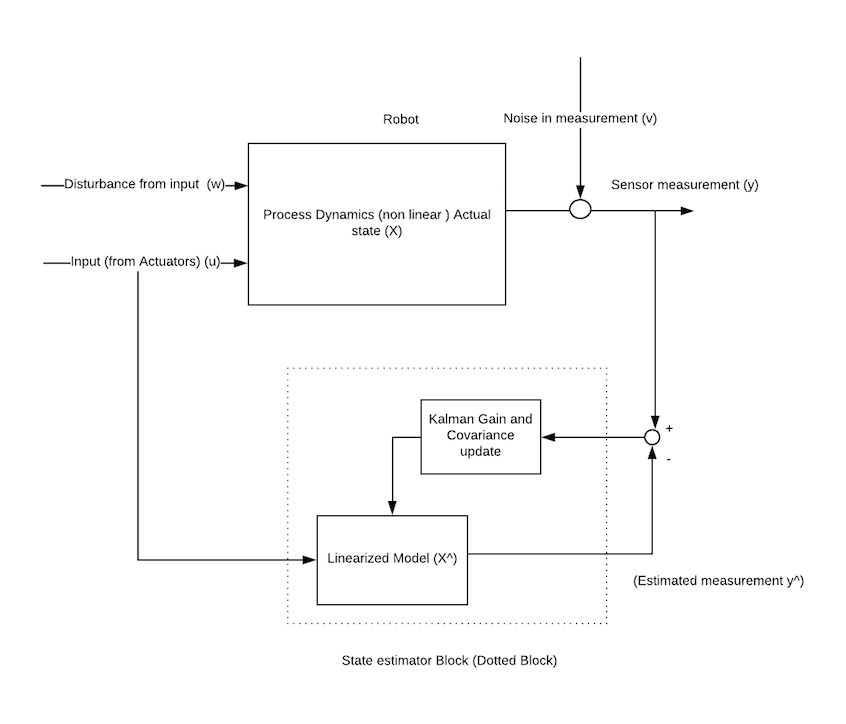
\includegraphics[width=110mm]{fig_1.png}
\caption{System Block Diagram}
\label{fig:figure1}
\end{figure}

Kalman filter would provide a linearized model of the robot.The point of this procedure is to minimize the difference between actual measurements and the filter approximations $(y-y\hat{})$ therefore with each iteration through the loop state of robot can be calculated with great accuracy.   
\\
\newpage
\section{Symbols}
Here is the list of all symbols we used for deriving Kalman filter in order to build state estimator:
\\
\begin{tabular}{c p{1\textwidth}}
  $L_x$ & length of the box  \\
  $L_y$ & width of the box \\
  $W$ & distance between rotating center and sensors center \\
  $C_v$ & coefficient, distance traveled by the wheel per unit of delay time \\
  $C_r$ & coefficient, body orientation changed by the wheel per unit of delay time \\
  $l_x$ & first range sensor reading (located on front of the car) \\
  $l_y$ & second range sensor reading (located on right side of the car) \\
  $\alpha$ & MPU angle measurement \\
  $r_x$ & absolute x coordinate of the car \\
  $r_y$ & absolute y coordinate of the car \\
  $\theta$ & absolute orientation of the car \\
  $\tau_L$ & Servo input: delay time of the left wheel \\
  $\tau_R$ & Servo input: delay time of the right wheel \\
  $\theta_{tht}$ & top half threshold angle \\
  $\theta_{thb}$ & bottom half threshold angle \\
  $\theta_{thr}$ & bottom right threshold angle \\
  $\theta_{thl}$ & bottom left threshold angle \\
  $\epsilon_{str}$ & picking variable, 1 if going straight line, 0 otherwise \\
  $w_t$ & process noise \\
  $v_t$ & measurement noise
\end{tabular}\\
\\ \\ \\ \\ \\ \\

\newpage
\section{Assumption}
For the sake of simplicity, we have the following assumption in the derivation below
\begin{enumerate}
\item $\theta$ takes value only (-90, 90)
\item $\tau_L$ and $\tau_R$ has the same magnitude, opposite sign if turning, otherwise same sign 
\item $\theta = \alpha$ assuming we have the the MPU calibrated at the 0 point
\end{enumerate}  



\begin{align*}
  \intertext{State}
  x = 
  \begin{bmatrix}
    r_x \\
    r_y \\
    \theta 
  \end{bmatrix} \\
  \intertext{Sensor Measurements}
  y = 
  \begin{bmatrix}
    l_x \\
    l_y \\
    \alpha
  \end{bmatrix} \\
  \intertext{Input}
  u = 
  \begin{bmatrix}
    \tau_L \\
    \tau_R
  \end{bmatrix} \\  
\end{align*}

\section{Sensor Measurement}
As shown in the picture below, $\theta$ is the angle the head of the car would have with respect to the direction of $L_x$. In order to do the calculations required there are four more threshold angles defined as tht (top), thb (bottom), thr (right) and thl(left). 
\begin{figure}[h!]
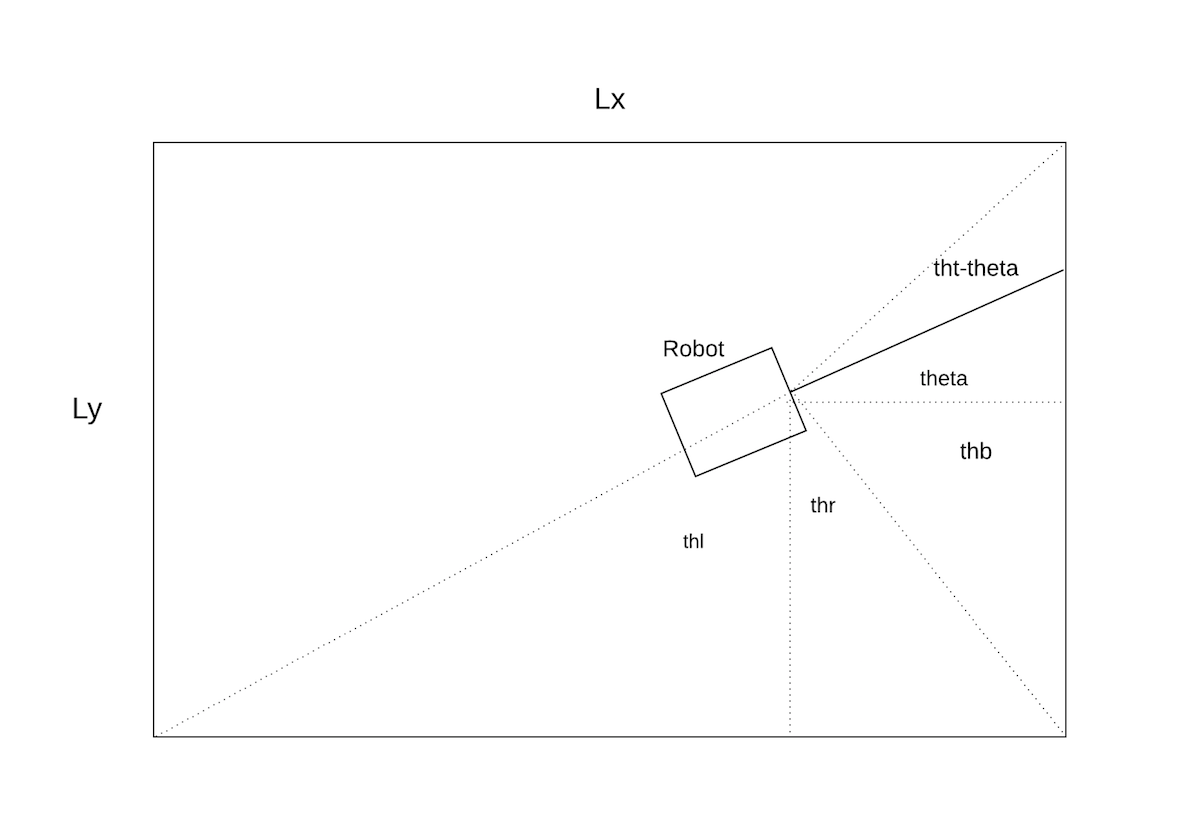
\includegraphics[width=110mm]{fig_2.png}
\caption{Threshold angles and theta ($\theta$)}
\label{fig:figure2}
\end{figure}
\\
\\
These angles are then used to find a function such that $y = h(x)$ \\
Threshold angles can be shown using trigonometry relationships:
\begin{align*}
  \theta_{tht} &= \tan^{-1}(\frac{L_y - r_y}{L_x - r_x}) \\
  \theta_{thb} &= \tan^{-1}(\frac{r_y}{L_x - r_x}) \\
  \theta_{thr} &= \tan^{-1}(\frac{L_x-r_x}{r_y}) \\
  \theta_{thl} &= \tan^{-1}(\frac{r_x}{r_y})
\end{align*}











Under mentioned assumption, the expression for $l_x$ (front range sensor reading) varies based on below four cases:
\begin{align*}
  l_x = \frac{L_x - r_x}{\cos \theta} \quad ,\quad 0 < \theta < \theta_{tht} \\
  l_x = \frac{L_y - r_y}{\sin \theta} \qquad  \theta > \theta_{tht} \\
  l_x = \frac{L_x - r_x}{\cos \theta} \quad \theta < 0, |\theta| < |\theta_{thb}| \\
  l_x = \frac{r_y}{\sin|\theta|} \quad \theta < 0, |\theta| > \theta_{thb}
\end{align*}
the expression for $l_y$ (right side sensor reading) varies under these four cases:
\begin{align*}
  l_y = \frac{r_y}{\cos |\theta|} \quad  ,\quad 0 < \theta < \theta_{thr} \\
  l_y = \frac{L_x - r_x}{\sin |\theta|} \qquad \theta > \theta_{thr} \\
  l_y = \frac{r_y}{\cos |\theta|} \quad \theta < 0, |\theta| < \theta_{thl} \\
  l_y = \frac{r_x}{\sin |\theta|} \quad \theta < 0, |\theta| > \theta_{thl}
\end{align*}
The derived expression for $\alpha = \theta$ doesn't change under the mentioned assumption. \par
\newpage
To summarize, there are total of 8 cases as indicated below:
\\
\begin{align*}
  \intertext{$\theta \geq 0, |\theta| < \theta_{tht}, |\theta| < \theta_{thr}$}
  y = 
  \begin{bmatrix}
    \frac{L_x - r_x}{\cos |\theta|} \\
    \frac{r_y}{\cos |\theta|} \\
    \alpha = \theta
  \end{bmatrix}
  \intertext{$\theta>0, |\theta| < \theta_{tht}, |\theta| > \theta_{thr}$}
  y = 
  \begin{bmatrix}
    \frac{L_x - r_x}{\cos |\theta|} \\
    \frac{L_x - r_x}{\sin |\theta|} \\
    \alpha = \theta
  \end{bmatrix}
  \intertext{$\theta>0, |\theta| > \theta_{tht}, |\theta| < \theta_{thr}$}
  y = 
  \begin{bmatrix}
    \frac{L_y - r_y}{\sin |\theta|} \\    
    \frac{r_y}{\cos |\theta|} \\
    \alpha = \theta
  \end{bmatrix}
  \intertext{$\theta>0, |\theta| > \theta_{tht}, |\theta| > \theta_{thr}$}
  y = 
  \begin{bmatrix}
    \frac{L_y - r_y}{\sin |\theta|} \\
    \frac{L_x - r_x}{\sin |\theta|} \\
    \alpha = \theta
  \end{bmatrix}
  %% \theta < 0
  \intertext{$\theta<0, |\theta| < \theta_{thb}, |\theta| < \theta_{thl}$}
  y = 
  \begin{bmatrix}
    \frac{L_x - r_x}{\cos |\theta|} \\
    \frac{r_y}{\cos |\theta|} \\
    \alpha = \theta
  \end{bmatrix}
  \intertext{$\theta<0, |\theta| < \theta_{thb}, |\theta| > \theta_{thl}$}
  y = 
  \begin{bmatrix}
    \frac{L_x - r_x}{\cos |\theta|} \\
    \frac{r_x}{\sin |\theta|} \\
    \alpha = \theta
  \end{bmatrix}
  \intertext{$\theta<0, |\theta| > \theta_{thb}, |\theta| < \theta_{thl}$}
  y = 
  \begin{bmatrix}
    \frac{r_y}{\sin |\theta|} \\    
    \frac{r_y}{\cos |\theta|} \\
    \alpha = \theta
  \end{bmatrix}
  \intertext{$\theta<0, |\theta| > \theta_{thb}, |\theta| > \theta_{thl}$}
  y = 
  \begin{bmatrix}
    \frac{r_y}{\sin |\theta|} \\        
    \frac{r_x}{\sin |\theta|} \\
    \alpha = \theta
  \end{bmatrix}  
\end{align*}
\\
\\
Now in order to obtain the model shown in Figure 1, all eight cases have to be linearized in order to derive matrix H where: $y = H x$. As for demonstratation purposes the linearization of case one where $\theta >0, |\theta| < \theta_{tht}, |\theta| < \theta_{thr}$, is shown:
\begin{align*}
  l_x &= \frac{L_x - r_x}{\cos \theta} \\
  l_y &= \frac{r_y}{\cos \theta} \\
  \intertext{Linearization around $l_{x0}, l_{y0}, \alpha_{0} = h(r_{x0}, r_{y0}, \theta_0)$}
  l_x &= l_{x0} + \frac{-1}{\cos \theta_0} (r_x - r_{x0}) + \frac{(L_x - r_{x0})\sin(\theta_0)}{(\cos{\theta_0})^2} (\theta - \theta_0) \\
  l_y &= l_{y0} + \frac{1}{\cos \theta_0}(r_y - r_{y0}) + \frac{r_{y0} \sin(\theta_0)}{(\cos \theta_0)^2} (\theta - \theta_0) \\
  l_x &= \frac{-1}{\cos \theta_0} r_x + \frac{(L_x - r_{x0})\sin(\theta_0)}{(\cos{\theta_0})^2} \theta + [\frac{r_{x0}}{\cos \theta_0} - \frac{(L_x - r_{x0})\sin(\theta_0)}{(\cos{\theta_0})^2}\theta_0 + l_{x0}] \\
  l_y &= \frac{1}{\cos \theta_0}r_y + \frac{r_{y0} \sin(\theta_0)}{(\cos \theta_0)^2} \theta + [\frac{-r_{y0}}{\cos \theta_0} - \frac{r_{y0} \sin(\theta_0)}{(\cos \theta_0)^2} \theta_0 + l_{y0}]
\end{align*}
In matrix form, the complete form for this case is
\begin{align*}
  y =
  \begin{bmatrix}
    \frac{-1}{\cos \theta_0} & 0 & \frac{(L_x - r_{x0})\sin(\theta_0)}{(\cos{\theta_0})^2} \\
    0 & \frac{1}{\cos \theta_0} & \frac{r_{y0} \sin(\theta_0)}{(\cos \theta_0)^2} \\
    0 & 0 & 1
  \end{bmatrix}
            \begin{bmatrix}
              r_x \\
              r_y \\
              \theta
            \end{bmatrix}
            +
            \begin{bmatrix}
              \frac{r_{x0}}{\cos \theta_0} - \frac{(L_x - r_{x0})\sin(\theta_0)}{(\cos{\theta_0})^2}\theta_0 + l_{x0} \\
              \frac{-r_{y0}}{\cos \theta_0} - \frac{r_{y0} \sin(\theta_0)}{(\cos \theta_0)^2} \theta_0 + l_{y0} \\
              0
            \end{bmatrix}
\end{align*}

\newpage
\section{Complete Case Analysis}
\begin{align*}
  \intertext{$\theta \geq 0, |\theta| < \theta_{tht}, |\theta| < \theta_{thr}$}
  H &= 
  \begin{bmatrix}
    \frac{-1}{\cos \theta_0} & 0 & \frac{(L_x - r_{x0})\sin(\theta_0)}{(\cos{\theta_0})^2} \\
    0 & \frac{1}{\cos \theta_0} & \frac{r_{y0} \sin(\theta_0)}{(\cos \theta_0)^2} \\
    0 & 0 & 1
  \end{bmatrix}
            \quad
            C =
            \begin{bmatrix}
              \frac{r_{x0}}{\cos \theta_0} - \frac{(L_x - r_{x0})\sin(\theta_0)}{(\cos{\theta_0})^2}\theta_0 + l_{x0} \\
              \frac{-r_{y0}}{\cos \theta_0} - \frac{r_{y0} \sin(\theta_0)}{(\cos \theta_0)^2} \theta_0 + l_{y0} \\
              0
            \end{bmatrix}            
  \intertext{$\theta \geq 0, |\theta| < \theta_{tht}, |\theta| > \theta_{thr}$}
  H &= 
  \begin{bmatrix}
    \frac{-1}{\cos \theta_0} & 0 & \frac{(L_x - r_{x0})\sin(\theta_0)}{(\cos{\theta_0})^2} \\
    \frac{-1}{\sin |\theta_0|} & 0 & -\frac{\theta_0}{|\theta_0|}\frac{L_x - r_{x0} \cos(\theta_0)}{(\sin |\theta_0|)^2} \\
    0 & 0 & 1
  \end{bmatrix}
            \quad
            C =
            \begin{bmatrix}
              \frac{r_{x0}}{\cos \theta_0} - \frac{(L_x - r_{x0})\sin(\theta_0)}{(\cos{\theta_0})^2}\theta_0 + l_{x0} \\
              \frac{r_{x0}}{\sin |\theta_0|} + \frac{(L_x - r_{x0}) \cos(\theta_0)}{(\sin |\theta_0|)^2} |\theta_0| + l_{y0} \\
              0
            \end{bmatrix}            
  \intertext{$\theta>0, |\theta| > \theta_{tht}, |\theta| < \theta_{thr}$}
  H &= 
  \begin{bmatrix}
    0 & \frac{-1}{\sin |\theta_0|} & -\frac{\theta_0}{|\theta_0|}\frac{L_y - r_{y0} \cos(\theta_0)}{(\sin |\theta_0|)^2} \\    
    0 & \frac{1}{\cos \theta_0} & \frac{r_{y0} \sin(\theta_0)}{(\cos \theta_0)^2} \\
    0 & 0 & 1
  \end{bmatrix}
            \quad
            C =
            \begin{bmatrix}
              \frac{r_{y0}}{\sin |\theta_0|} + \frac{(L_y - r_{y0}) \cos(\theta_0)}{(\sin |\theta_0|)^2} |\theta_0| + l_{x0} \\              
              \frac{-r_{y0}}{\cos \theta_0} - \frac{r_{y0} \sin(\theta_0)}{(\cos \theta_0)^2} \theta_0 + l_{y0} \\
              0
            \end{bmatrix}              
  \intertext{$\theta>0, |\theta| > \theta_{tht}, |\theta| > \theta_{thr}$}
  H &= 
  \begin{bmatrix}
    0 & \frac{-1}{\sin |\theta_0|} & -\frac{\theta_0}{|\theta_0|}\frac{L_y - r_{y0} \cos(\theta_0)}{(\sin |\theta_0|)^2} \\
    \frac{-1}{\sin |\theta_0|} & 0 & -\frac{\theta_0}{|\theta_0|}\frac{L_x - r_{x0} \cos(\theta_0)}{(\sin |\theta_0|)^2} \\    
    0 & 0 & 1
  \end{bmatrix}
            \quad
            C =
            \begin{bmatrix}
              \frac{r_{y0}}{\sin |\theta_0|} + \frac{(L_y - r_{y0}) \cos(\theta_0)}{(\sin |\theta_0|)^2} |\theta_0| + l_{x0} \\
              \frac{r_{x0}}{\sin |\theta_0|} + \frac{(L_x - r_{x0}) \cos(\theta_0)}{(\sin |\theta_0|)^2} |\theta_0| + l_{y0} \\              
              0
            \end{bmatrix}                
  %% \theta < 0
  \intertext{$\theta<0, |\theta| < \theta_{thb}, |\theta| < \theta_{thl}$}
  H &= 
  \begin{bmatrix}
    \frac{-1}{\cos \theta_0} & 0 & \frac{(L_x - r_{x0})\sin(\theta_0)}{(\cos{\theta_0})^2} \\
    0 & \frac{1}{\cos \theta_0} & \frac{r_{y0} \sin(\theta_0)}{(\cos \theta_0)^2} \\
    0 & 0 & 1
  \end{bmatrix}
            \quad
            C =
            \begin{bmatrix}
              \frac{r_{x0}}{\cos \theta_0} - \frac{(L_x - r_{x0})\sin(\theta_0)}{(\cos{\theta_0})^2}\theta_0 + l_{x0} \\
              \frac{-r_{y0}}{\cos \theta_0} - \frac{r_{y0} \sin(\theta_0)}{(\cos \theta_0)^2} \theta_0 + l_{y0} \\
              0
            \end{bmatrix}              
  \intertext{$\theta<0, |\theta| < \theta_{thb}, |\theta| > \theta_{thl}$}
  H &= 
  \begin{bmatrix}
    \frac{-1}{\cos \theta_0} & 0 & \frac{(L_x - r_{x0})\sin(\theta_0)}{(\cos{\theta_0})^2} \\
    \frac{1}{\sin |\theta_0|} & 0 & -\frac{\theta_0}{|\theta_0|}\frac{r_{x0} \cos(\theta_0)}{(\sin |\theta_0|)^2} \\
    0 & 0 & 1
  \end{bmatrix}
            \quad
            C =
            \begin{bmatrix}
              \frac{r_{x0}}{\cos \theta_0} - \frac{(L_x - r_{x0})\sin(\theta_0)}{(\cos{\theta_0})^2}\theta_0 + l_{x0} \\
              \frac{-r_{x0}}{\sin |\theta_0|} + \frac{r_{x0} \cos(\theta_0)}{(\sin |\theta_0|)^2} |\theta_0| + l_{y0} \\
              0
            \end{bmatrix}              
  \intertext{$\theta<0, |\theta| > \theta_{thb}, |\theta| < \theta_{thl}$}
  H &= 
  \begin{bmatrix}
    0 & \frac{1}{\sin |\theta_0|} & -\frac{\theta_0}{|\theta_0|}\frac{r_{y0} \cos(\theta_0)}{(\sin |\theta_0|)^2} \\    
    0 & \frac{1}{\cos \theta_0} & \frac{r_{y0} \sin(\theta_0)}{(\cos \theta_0)^2} \\
    0 & 0 & 1
  \end{bmatrix}
            \quad
            C =
            \begin{bmatrix}
              -\frac{r_{y0}}{\sin |\theta_0|} + \frac{r_{y0} \cos(\theta_0)}{(\sin |\theta_0|)^2} |\theta_0| + l_{x0} \\              
              \frac{-r_{y0}}{\cos \theta_0} - \frac{r_{y0} \sin(\theta_0)}{(\cos \theta_0)^2} \theta_0 + l_{y0} \\
              0
            \end{bmatrix}                
  \intertext{$\theta<0, |\theta| > \theta_{thb}, |\theta| > \theta_{thl}$}
  H &= 
  \begin{bmatrix}
    0 & \frac{1}{\sin |\theta_0|} & -\frac{\theta_0}{|\theta_0|}\frac{r_{y0} \cos(\theta_0)}{(\sin |\theta_0|)^2} \\
    \frac{1}{\sin |\theta_0|} & 0 & -\frac{\theta_0}{|\theta_0|}\frac{r_{x0} \cos(\theta_0)}{(\sin |\theta_0|)^2} \\    
    0 & 0 & 1
  \end{bmatrix}
            \quad
            C =
            \begin{bmatrix}
              -\frac{r_{y0}}{\sin |\theta_0|} + \frac{r_{y0} \cos(\theta_0)}{(\sin |\theta_0|)^2} |\theta_0| + l_{x0} \\
              -\frac{r_{x0}}{\sin |\theta_0|} + \frac{r_{x0} \cos(\theta_0)}{(\sin |\theta_0|)^2} |\theta_0| + l_{y0} \\              
              0
            \end{bmatrix}                  
\end{align*}


\section{State Evolution}
The goal for this section is to find a function such that $x_{t+1} = f(x_{t}, u_{t})$. 
\par
To begin with, there are two cases to consider:
\begin{align*}
  \intertext{Case 1: the car is going in a straight line (either backward or forward): $(\tau_{L,t} * \tau_{R,t}) > 0$}
  r_{x,t+1} &= r_{x,t} + C_v * \tau_{R,t} \cos \theta \\
  r_{y,t+1} &= r_{y,t} + C_v * \tau_{R,t} \sin \theta \\
  \theta_{th1} &= \theta_t
  \intertext{Case 2: the car is turning (either left or right): $(\tau_{L,t} * \tau_{R,t}) > 0$}
  r_{x,t+1} &= r_{x,t} - W[1 - \cos(C_r\tau_{R,t})]\\
  r_{y,t+1} &= r_{y,t} + W[\sin{(C_{r}\tau_{R,t})}]\\
  \theta_{th1} &= \theta_t + C_r \tau_{R, t}
                 \intertext{notice that all the signs worked out in the above expressions either going forward or backward, or turning left or right}
\end{align*}
To combine these two cases into one expression, we define a picking variable $\epsilon_{str} = \tau_{L,t} * \tau_{R,t} > 0)$ taking value 0 or 1. Then,
\begin{align*}
  r_{x,t+1} &= r_{x,t} + \epsilon_{str} * C_v \tau_{R,t} \cos \theta - (1-\epsilon_{str})*W[1 - \cos(C_r\tau_{R,t})]\\
  r_{y,t+1} &= r_{y,t} + \epsilon_{str} * C_v \tau_{R,t} \sin \theta + (1-\epsilon_{str})*W[\sin{(C_{r}\tau_{R,t})}]\\
  \theta_{th1} &= \theta_t + (1 - \epsilon_{str}) * C_r \tau_{R,t} \\
  \intertext{In matrix form,}
  x_{t+1} &=
            \begin{bmatrix}
              1 & 0 & 0 \\
              0 & 1 & 0 \\
              0 & 0 & 1
            \end{bmatrix}
            \begin{bmatrix}
              r_{x,t} \\
              r_{y,t} \\
              \theta_t
            \end{bmatrix}
            +
            \begin{bmatrix} 
              0 & \epsilon_{str} C_v \cos \theta_t \\
              0 & \epsilon_{str} C_v \sin \theta_t \\
              0 & (1 - \epsilon_{str}) C_r \\    
            \end{bmatrix}
  \begin{bmatrix}
    \tau_{L, t} \\
    \tau_{R, t}
  \end{bmatrix} \\
  x_{t+1} &= A x_{t} + B_t u_{t}
\end{align*}

\newpage
\section{Kalmen Filter Procedure}
\subsection{Kalman Gain Update}
\begin{enumerate}
\item Initial Error Covariance $P_{1|0} = P_0, t = 1$
\item Compute Gain: $K_t = P_{t|t-1} H_t^T [H_t^T P_{t|t-1} H_t^T + R_t]^{-1}$
\item Update error covariance
  \begin{enumerate}
  \item $P_t = (I-K_tH_t)P_{t|t-1}$
  \item $P_{t+1|t} = A_t P A_t^T + G_t Q_t G_t^T$
  \end{enumerate}
\item t = t+1
\item Go back to (2) until stop condition
\end{enumerate}
where
\begin{align*}
  R_t &= E[v_t v_t^T] \\
  Q_t &= E[w_t w_t^T]
\end{align*}

\subsection{State Estimation}
\begin{enumerate}
\item Initialize estimated state $\hat{x}_0$
\item Collect new measurement $y_t$
\item Update State Estimate with new measurement, with updated Kalman gain from above
  \begin{enumerate}
  \item $\hat{x}_{t|t-1} = A_{t-1} \hat{x}_{t-1}$ 
  \item $\hat{x}_t = \hat{x}_{t|t-1} + K_t(y_t - H_t \hat{x}_{t|t-1})$
  \end{enumerate}
\item t = t+1
\item Go back to (2) until stop condition  
\end{enumerate}
\newpage
\section{Demonstration}
Explain the condition and cases tested in our computer and actual outfield demo and put the youtube links to both here:
1. ... \\2. ...
\subsection{Communication method used on robot}
In this final section the compatibility of the simulation code with the robot is explained. Now here is a brief summary of the method of communication used in this lab. \\ 
State estimation code is run on a personal computer and all the simulation is done in the matlab software. ESP8266 WIFI module chip is used to create an access point. The PC then is connected to ESP access point in order to receive, process and transfer data back to ESP. The format of data transferred back and forth is Json which makes the data extraction on each end very simple. In order to send Json from ESP MIT ArduinoJson library was used. 

\begin{figure}[h!]
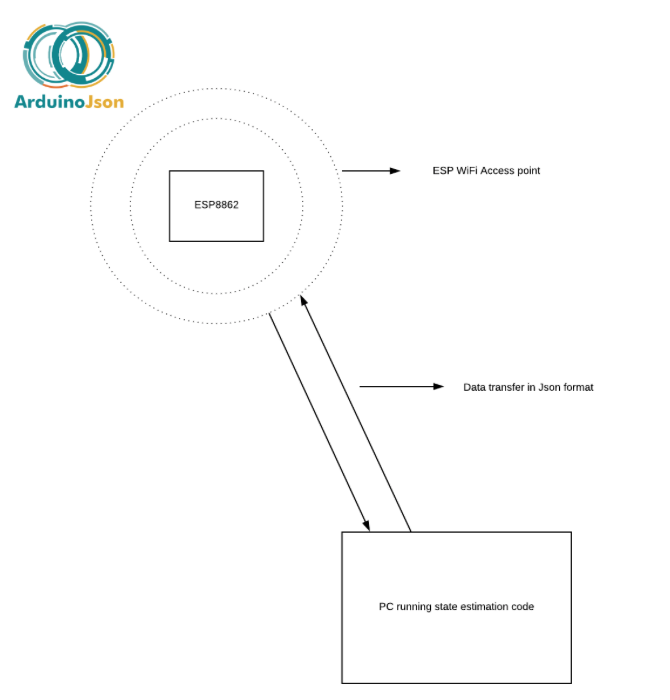
\includegraphics[width=110mm]{fig_3.png}
\caption{Communication diagram}
\label{fig:figure3}
\end{figure}
   
\end{document}

%==================================================%
% Bibliography starts here
%==================================================%
% \bibliographystyle{unsrt}
% \bibliography{my_latex_math_template}

%%% Local Variables:
%%% mode: latex
%%% TeX-master: t
%%% End:
